\chapter{Servidor web de imágenes mediante ROS }\label{cap.camserver}
En este capítulo expondrá la creación de un nuevo driver para la plataforma JdeRobot. Este driver será un servidor de imágenes al que se ha llamado camServerWeb, obtenidas mediante una webcam (ya sea externa o interna del ordenador) de modo que cualquier aplicación externa pueda obtener las imágenes obtenidas.
\section{Introducción e infraestructura}
Este driver está diseñado con JavaScript y HTML como lenguajes de programación, y ROS como middleware para la interconexión con los diferentes clientes. La imagen 4.1 muestra un esquema de funcionamiento.
\begin{figure}[H]
  \begin{center}
    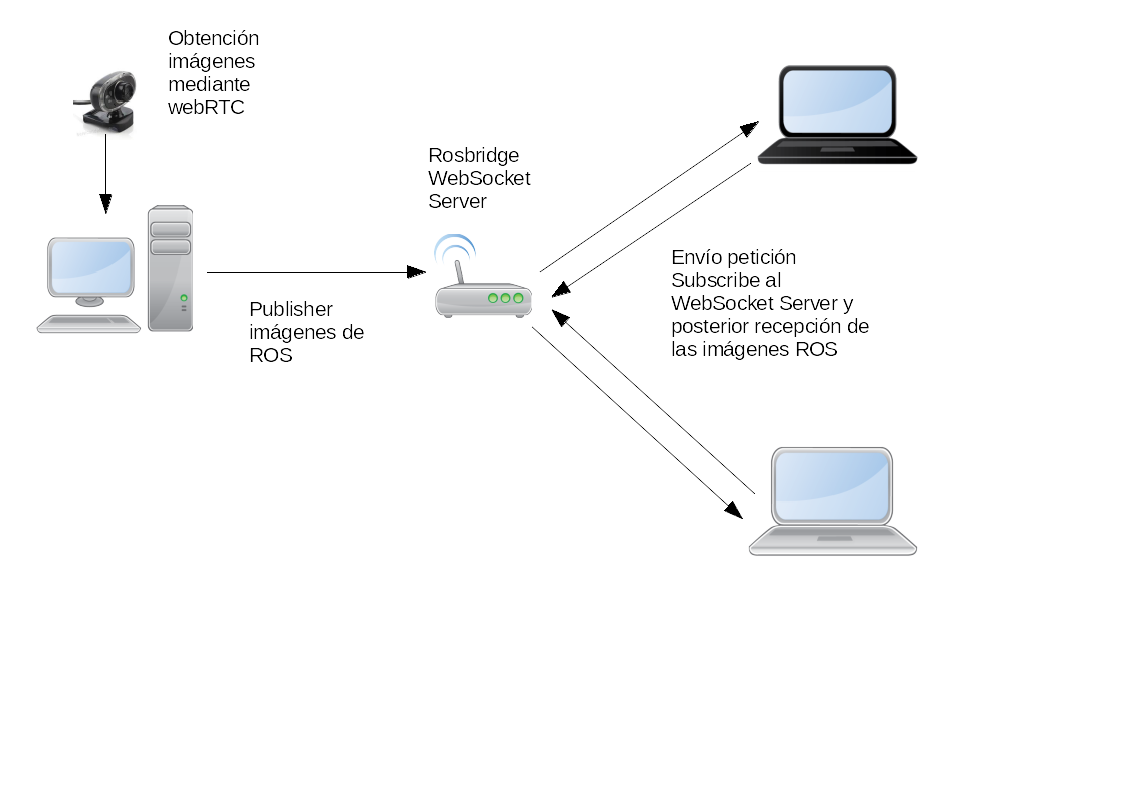
\includegraphics[width=0.8\textwidth]{figures/esquemacamserver.png}
		\caption{Esquema del funcionamiento del servidor de imagenes}
		\label{fig.esquemacamserver}
		\end{center}
\end{figure}
La imagen se obtiene de la webcam de la que se desee (por defecto se selecciona la webcam interna del ordenador) mediante webRTC. Esta imagen se transmite mediante el middleware ROS utilizando el modelo Publicador/Subscriptor. El driver será el Publicador, y lo hará estableciendo un topic o etiqueta y usando las imágenes comprimidas de ROS (CompressedImage). Dado que, como se ha explicado en los capítulos anteriores, ROS no ofrece soporte por defecto para JavaScript, se usa roslibjs.
Una vez se ha comenzado a publicar las imágenes, cualquier aplicación que se subscriba al topic, podrá recibirlas, dando igual el lenguaje de programación o sistema operativo que utilice.
El driver se divide en tres partes, una primera parte que es la interfaz gráfica, una segunda que es la conexión y obtención de las imágenes, y la tercera y última que es la correspondiente a la transmisión mediante ROS.
\section{Interfaz gráfica}
Dado que es un driver y su cometido no es mostrar nada, la interfaz gráfica que se ha creado es muy simple. En ella únicamente se mostrara si está conectado y a la IP y Puerto al que lo está. 
La interfaz está realizada mediante HTML y Bootstrap, siguiendo el modelo del resto de aplicaciones web de la plataforma JdeRobot.
\begin{figure}[H]
  \begin{center}
    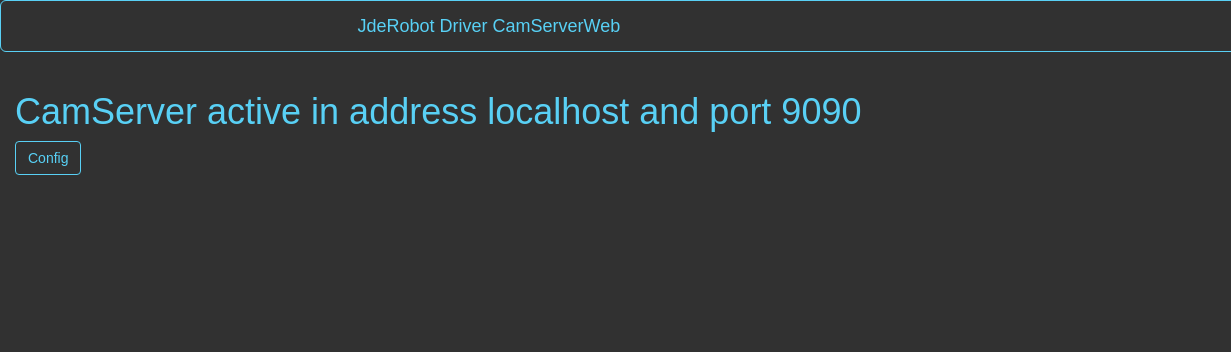
\includegraphics[width=0.8\textwidth]{figures/Interfazcamserver.png}
		\caption{Interfaz gráfica del driver}
		\label{fig.interfazcamserver}
		\end{center}
\end{figure}
La única funcionalidad destacable de la interfaz y el motivo para que haya sido necesario aportar una interfaz, es el menú de configuración. En este menú el usuario establecerá la IP y el puerto por el que se va a transmitir los mensajes, el topic al que se deberán subscribir los clientes y el tipo de mensajes, y la cámara de la que queremos obtener las imágenes que, como se indica anteriormente, por defecto será la interna del ordenador.
 \begin{figure}[H]
  \begin{center}
    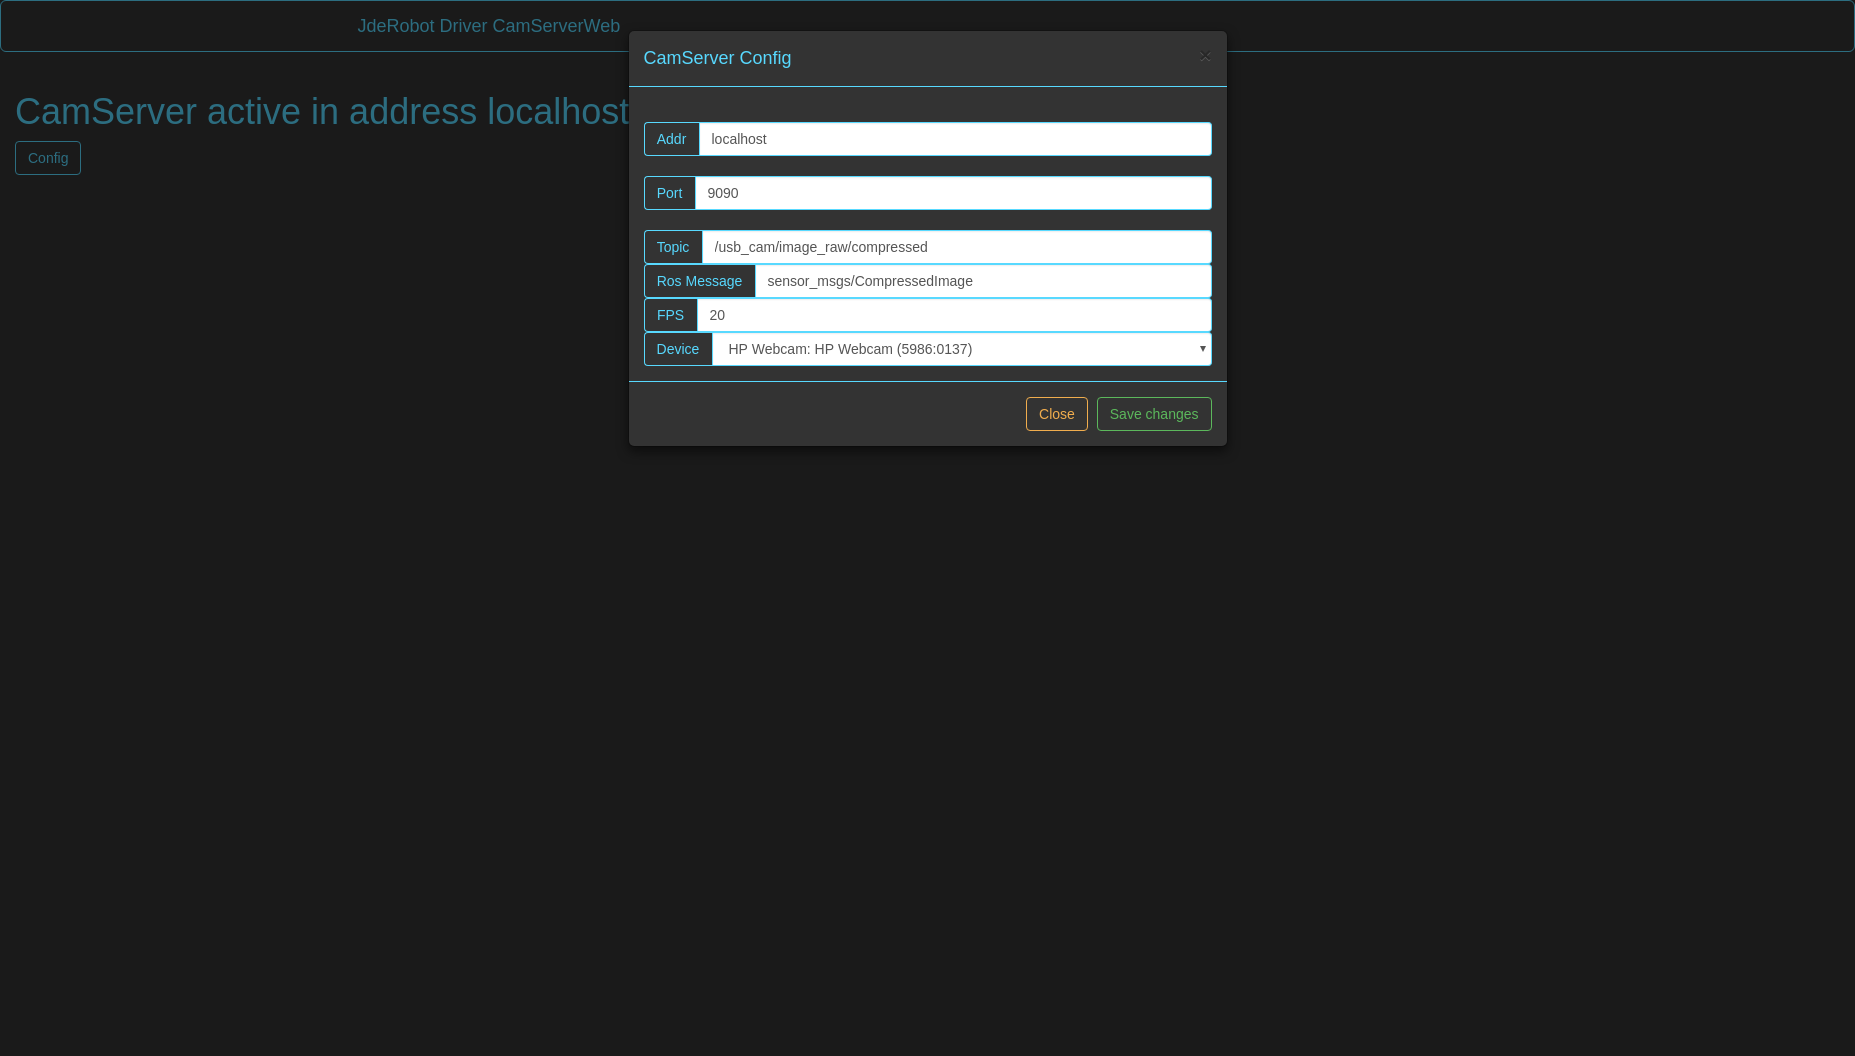
\includegraphics[width=0.8\textwidth]{figures/configcamserver.png}
		\caption{Menu de configuración del servidor de imagenes}
		\label{fig.configcamserver}
		\end{center}
\end{figure}

\section{Adquisición de las imágenes}
Para la obtención de las imágenes, como se ha indicado anteriormente, se hace uso del proyecto de código abierto webRTC, que nos permite la transmisión en tiempo real de audio, video y datos.
Mediante webRTC, obtenemos las imágenes de una cámara utilizando muy pocas línea de código, lo que nos facilita enormemente el trabajo. El único problema que se ha tenido que tener en cuenta y solucionar, es el formato en el que se obtienen esas imágenes que es incompatible con ROS, por lo que se han tenido que llevar a cabo modificaciones en el formato de la imagen.

Lo primero que se debe realizar es recopilar todos los dispositivos conectados al ordenador y separar los dispositivos de video, que son los que realmente nos interesan. Para lograrlo, se utiliza el api Navigator de webRTC, proporcionándonos el objeto navigator.mediaDevices, al cual si le añadimos .enumerateDevices().then(function (devices)\{\}, obtenemos todos los dispositivos multimedia conectados al ordenador donde se esta ejecutando. Una vez que ya tenemos todos los dispositivos, simplemente nos interesan como se ha indicado anteriormente, aquellos dispositivos capturadores de video, es decir serán aquellos dispositivos cuyo tipo es de entrada de video (en nuestro código sería un condicional if (devices.kind == "videoinput"\{\}). La lista de dispositivos se mostrara en el menu de configuración, mostrado en la sección anterior, mediante un campo desplegable como se muestra en la siguiente imagen:
 \begin{figure}[H]
  \begin{center}
    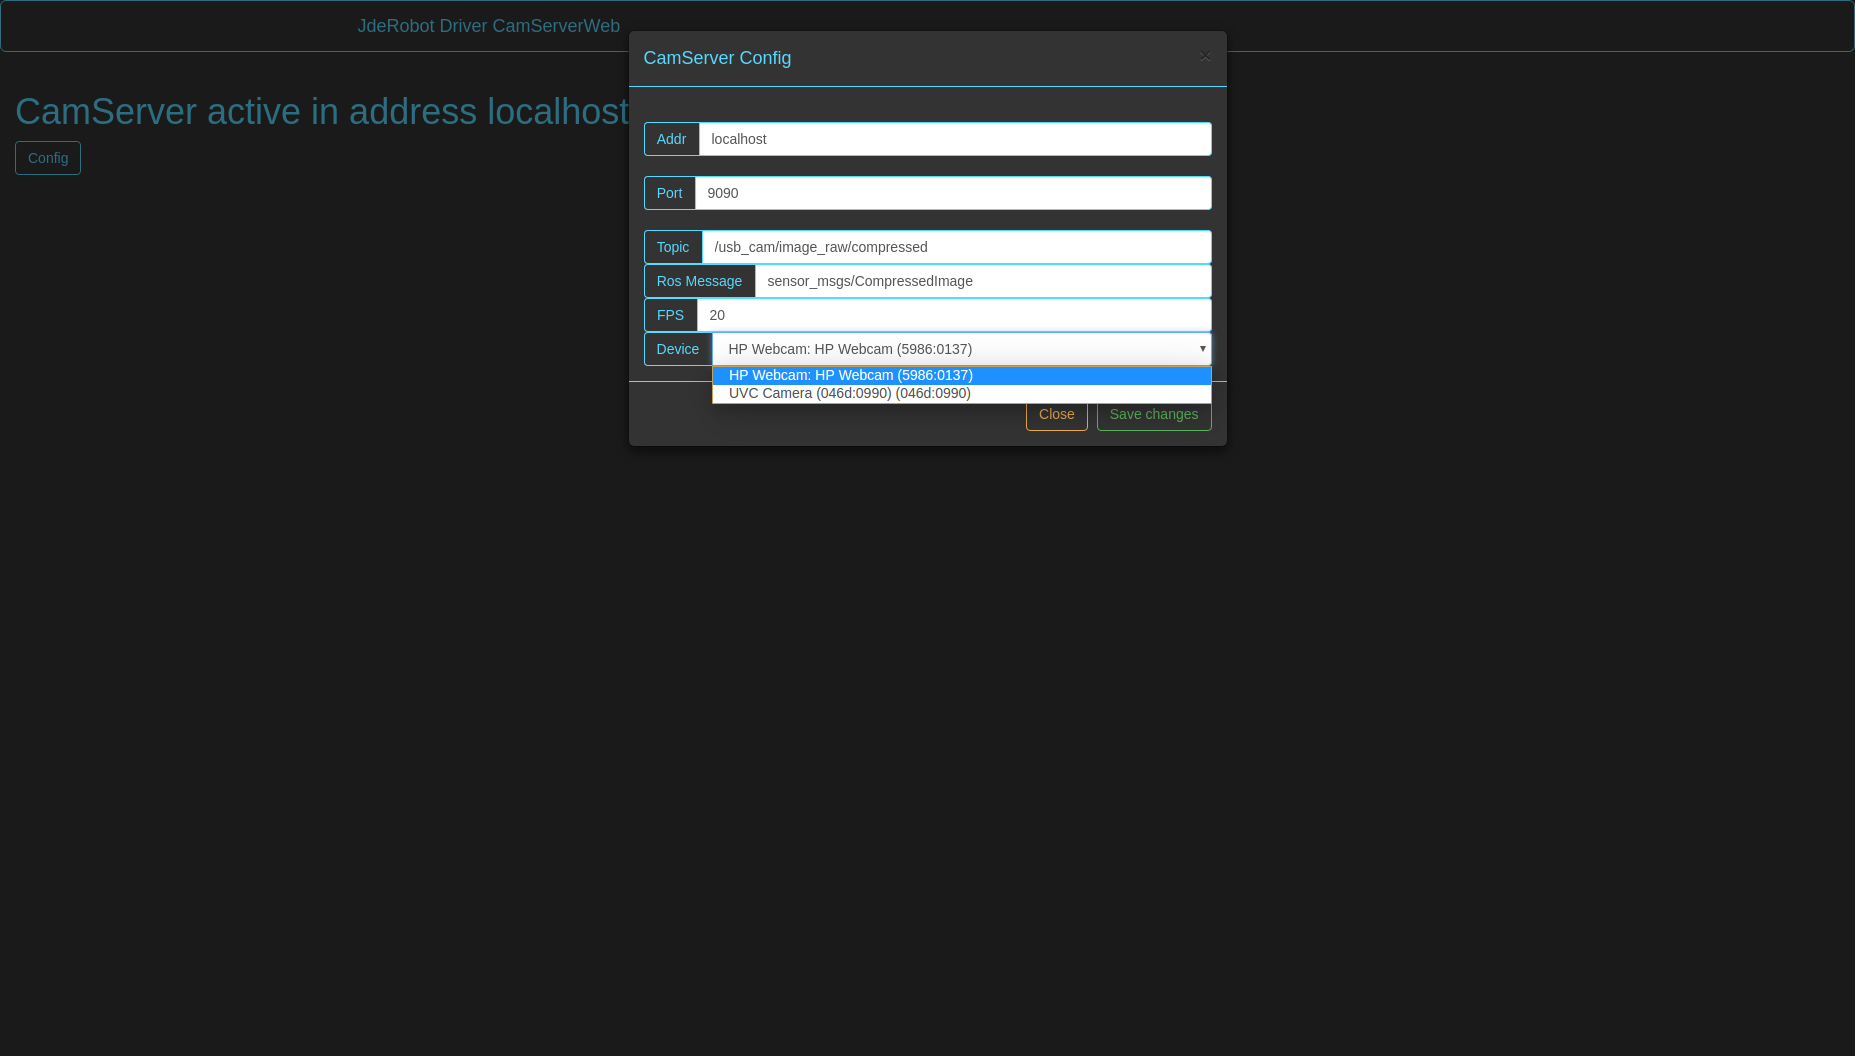
\includegraphics[width=0.8\textwidth]{figures/devicecamserver.png}
		\caption{Selector del dispositivo de entrada de video}
		\label{fig.devicecamserver}
		\end{center}
\end{figure}
Una vez que seleccionamos el dispositivo que vamos a utilizar para adquirir las imágenes, hay que conectarse a él. Para esta conexión, volvemos a utilizar la API de webRTC, Navigator y el objeto Navigator.mediaDevices, sin embargo en esta ocasión utilizamos el método navigator.mediaDevices.getUserMedia(constraints).then(function(stream) \{\}), donde constraints define los dispositivos multimedia (en este caso el dispositivo de entrada de video escogido) y stream es el flujo de datos obtenido de ellos.
Este flujo de datos esta en el formato MediaStream, el cual no es apto para ser enviado o visualizado, por tanto es necesario realizar una reconversión. Para realizar al reconversión, vamos a utilizar el elemento de HTML canvas y el método JavaScript asociado a este elemento toDataURL(). Este método nos devuelve un data URI (URLs prefijados que permiten a los creadores de contenido incorporar pequeños archivos en linea en los documentos) que contiene una representación de la imagen en el formato especificado por el parámetro type, tomando en nuestro caso el valor "image/jpeg", para obtener las imágenes en el formato comprimido jpeg. Todo esto estará contenido en un canvas virtual, ya que no se mostrara en ningún lugar y únicamente se utilizara como pasarela entre el API de webRTC y el envío de las imágenes.

\section{Conexión y transmisión de las imágenes mediante ROS}
En esta sección se explicara cómo realizar la  conexión a ROS y el posterior envío de imágenes mediante un Publisher de ROS. Como se indica en los capítulos anteriores, dado la limitación y la política de privacidad las tecnologías web, es necesario la existencia de un servidor intermedio que estará escuchando en una dirección IP y en un Puerto determinado, y hará las funciones de control de acceso y encaminamiento.

\subsection{Establecer conexión con ROS}
Para realizar la conexión es necesario el uso de la biblioteca roslibjs y que se ha explicado en capítulos anteriores. Esta biblioteca nos proporciona todo el código necesario para realizar la conexión, indicándonos si se ha realizado correctamente o a si ha ocurrido algún error. Para realizar la conexión, la biblioteca roslibjs nos proporciona el objeto ROSLIB.Ros, y el método proporcionado por este objeto, ros.on. El código para establecer la conexión queda como sigue:
\begin{lstlisting}[frame=single]
ros = new ROSLIB.Ros();
ros = new ROSLIB.Ros({
            url : "ws://IP:Puerto"
 });
\end{lstlisting}
En este código, indicaremos que la conexión se hará utilizando un canal de comunicación WebSocket, y la IP y puerto por la que se transmitirá. De esta forma ya habremos establecido la conexión ROS, pero aún deberemos definir el tipo de mensaje a enviar y a través de que etiqueta de ROS (topic de ROS) nos pueden localizar los clientes que deseen obtener lo que nuestro servidor de imágenes esta transmitiendo.

\subsection{Definición de los mensajes ROS}
El tipo de mensaje que vamos a utilizar para el envío sera el tipo predefinido en el API de ROS, "sensor\_msgs/CompressedImage". El motivo de la elección de este tipo es debido a que las imágenes se obtienen en formato comprimido "jpeg", tal y como se ha explicado en la sección anterior. Sin embargo, este tipo de mensaje no envía información acerca del tamaño de la imagen (altura y anchura), por lo que es necesario enviar otro mensaje adicional para completar esta información. Este mensaje de apoyo será de tipo "sensor\_msgs/CameraInfo" y transmitirá toda la información sobre la cámara (frames por segundo, altura, anchura, etc). Para definir estos dos mensajes, se utiliza el objeto proporcionado por la biblioteca roslibjs, ROSLIB.Topic. A este objete se le deben introducir como parámetros el objetos ROSLIB.Ros generado para realizar la conexión, el nombre del topic y el tipo de mensaje, por lo que generaremos nuestro Publisher para servir las imágenes (el Publisher para la información de la cámara sera similar) mediante el siguiente código:
\begin{lstlisting}[frame=single]
var imagenTopic = new ROSLIB.Topic({
	ros:ros, 
	name: "mi_servidor_imagenes", 
	messageType : "sensor_msgs/CompressedImage Message"})

\end{lstlisting}

\subsection{Creación de los mensajes y publicación}
Definidos los mensajes y establecida la conexión, el siguiente paso es transmitir los mensajes. Para ello se deben crear los mensajes con la información que deseamos transmitir con el Publisher, utilizando de nuevo un objeto definido en la biblioteca roslibjs, new ROSLIB.Message. Para crear este objeto, debemos pasar por parámetros el contenido que queramos que tenga nuestro mensaje, siempre cumpliendo las especificaciones definidas para cada tipo de mensaje escogidos anteriormente y que están definidas en la documentación de ROS  \footnote{\url{http://wiki.ros.org/common_msgs}}. En nuestro caso, para definir los dos mensajes que transmitiremos lo haremos mediante el siguiente código para el caso de la transmisión de las imágenes:
\begin{lstlisting}[frame=single]
 var videomensaje = new ROSLIB.Message({
 	format : "jpeg", 
	data : data.replace("data:image/jpeg;base64,", "")
	})

\end{lstlisting}
De el anterior código cabe destacar que data corresponde a los datos obtenidos mediante el método toDataURL indicado anteriormente, remplazando la cabecera donde se indica el formato, ya que el formato ya se indica en el propio mensaje mediante format.  Para el mensaje donde se transmite la información de la cámara usaremos el siguiente código:

\begin{lstlisting}[frame=single]
var camarainfo = new ROSLIB.Message({
	height: imagen.height,
	width: imagen.width})

\end{lstlisting}
Creados los mensajes, solo nos falta publicarlos, lo que se consigue de una manera sencilla mediante
\begin{lstlisting}[frame=single]
imageTopic.publish(imageMessage);
cameraInfo.publish(infoMessage);
\end{lstlisting}
Se puede apreciar fácilmente que lo que estamos haciendo es publicar los dos mensajes creados mediante la estructura definida anteriormente. 
Finalmente, es necesario enviar de una manera periódica estos mensajes, ya que con lo indicado anteriormente, únicamente estamos enviando un mensaje de cada. Para crear un envió periódico, se hace uso del método de JavaScript SetInterval(). Este método llama a una función o evalúa una expresión cuando pase un intervalo de tiempo (en milisegundos), que se indica en la llamada al método junto a la función que se quiere ejecutar cuando se cumpla el citado intervalo.
\section{Adaptación para su funcionamiento con Electron}
Hacer funcionar el servidor de imágenes con Electron es muy simple, únicamente deberemos generar un archivo JavaScript, que sera el encargado de generar la ventana y mostrar el fichero HTML que contendrá la interfaz gráfica, y crear el archivo package.json.
\subsection{package.json}
Como se indico en capítulos anteriores, Electron funciona bajo Node.js y su gestor de paquetes, npm, este hecho, nos obliga a que tengamos que generar este archivo package.json. El cometido del mismo será definir las dependecnais de paquetes de terceros que tendrá nuestro driver, definir las características de nuestro drivern (nombre, versión, autor, etc.) y, lo que es más importante, de que manera se lanzara nuestra driver y el archivo que se debe ejecutar al lanzarla. En el caso del servidor de imágenes, la dependencia será con Electron (tiene más dependencias pero no son vitales para su ejecución), el archivo principal, al que se ha nombrado como "main.js", será el encargado de generar la ventana, tal y como hemos indicado anteriormente, y se lanzara a través del framework Electron. Por lo tanto, el package.json quedará como sigue:
\begin{lstlisting}[frame=single]
{
  "name": "CamServerWeb",
  "version": "0.1.0",
  "main": "main.js",
  "scripts": {
    "start": "electron ."
  },
  "dependencies": {
      "electron": "^1.8.4",
  }
}
\end{lstlisting}
\subsection{main.js}
El archivo "main.js" indicado anteriormente, contendrá muy pocas lineas de código al tratarse de un elemento totalmente externo a nuestra driver y no tener ningún papel en el funcionamiento de el driver, únicamente es necesario para ejecutar el driver utilizando Electron. A continuación se muestra el código de este archivo:
\begin{lstlisting}[frame=single]
const app = require('electron')
const path = require('path')
const url = require('url')

let win;

function createWindow () {
  win = new BrowserWindow({width: 1800, height: 1000})
  win.loadURL(url.format({
    pathname: path.join(__dirname, 'camserver.html'),
    protocol: 'file:',
  }))
  
app.on('ready', createWindow)

\end{lstlisting}
Lo primero que se realiza es definir los módulos que se requieren para que funcione correctamente y que se utilizaran en el resto del código. Posteriormente, se define el tamaño de la ventana, en este caso la ventana sera de 1800 pixeles de ancho y 1000 de alto. Mediante win.loadURL se simula el funcionamiento de un navegador y como gestionan las diferentes URLs, este método se le pasara como parámetros el archivo HTML principal de nuestra driver, en otras palabras, el archivo HTML que activa el funcionamiento de el driver al contener la lógica de la misma, el protocolo que este caso es "file:", al estar queriendo mostrar directamente de un archivo HTML (si quisiéramos mostrar mediante Electron el contenido de una página web ya existente, protocol tomaría el valor "http:"). Finalmente, la última de código llamara a la función que crea la ventana y muestra el HTML en el momento que Electron haya terminado de inicializarse y esta preparado para la creación de la ventana.

\section{Ejecución del servidor de imagenes}
Como hemos visto anteriormente, el driver puede ejecutarse a través de dos vías: Electron y Node.js. Sin embargo, la preparación para que funcione correctamente es la misma para ambas vías, siendo la única diferencia la forma de ejecutar el driver.
En un primer terminal o consola se debe ejecutar el servidor intermedio de ROS explicado en capítulos anteriores.
\begin{lstlisting}[frame=single]
roslaunch rosbridge_server rosbridge_websocket.launch
\end{lstlisting}
El segundo terminal será donde lanzamos el driver, por lo que tenemos dos formas de hacerlo:
\begin{itemize}
\item 
Con Node.js
\end{itemize}
\begin{lstlisting}[frame=single]
node run.js
Arrancamos nuestro navegador favorito y ponemos la url http://localhost:7777/
\end{lstlisting}
\begin{itemize}
\item 
Con Electron
\end{itemize}
\begin{lstlisting}[frame=single]
npm install
npm start
\end{lstlisting}
En ambos casos debemos configurar el driver para que se conecte con el servidor intermedio, en la imagen 4.5 muestra una posible configuración del driver.
\begin{figure}[H]
  \begin{center}
    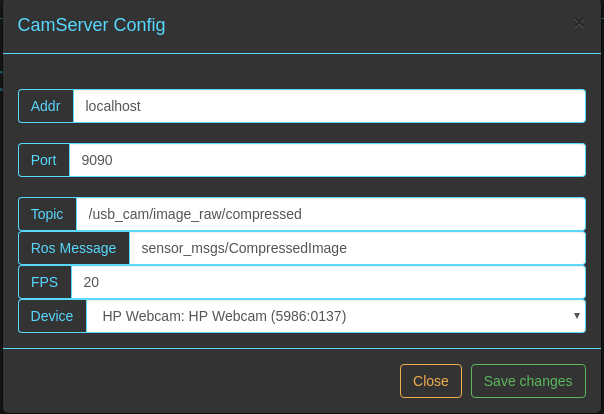
\includegraphics[width=0.8\textwidth]{figures/configcamservertest.png}
		\caption{Ejemplo de configuración del driver}
		\label{fig.esquemacamserver}
		\end{center}
\end{figure}
Finalmente, para verificar que esta funcionando correctamente, en un tercer terminal lanzaremos la herramienta rqt\_image\_view, facilitada por ROS para visualizar imágenes enviadas a través de un mensaje de ROS.
\begin{figure}[H]
  \begin{center}
    \subfigure[Node.js]{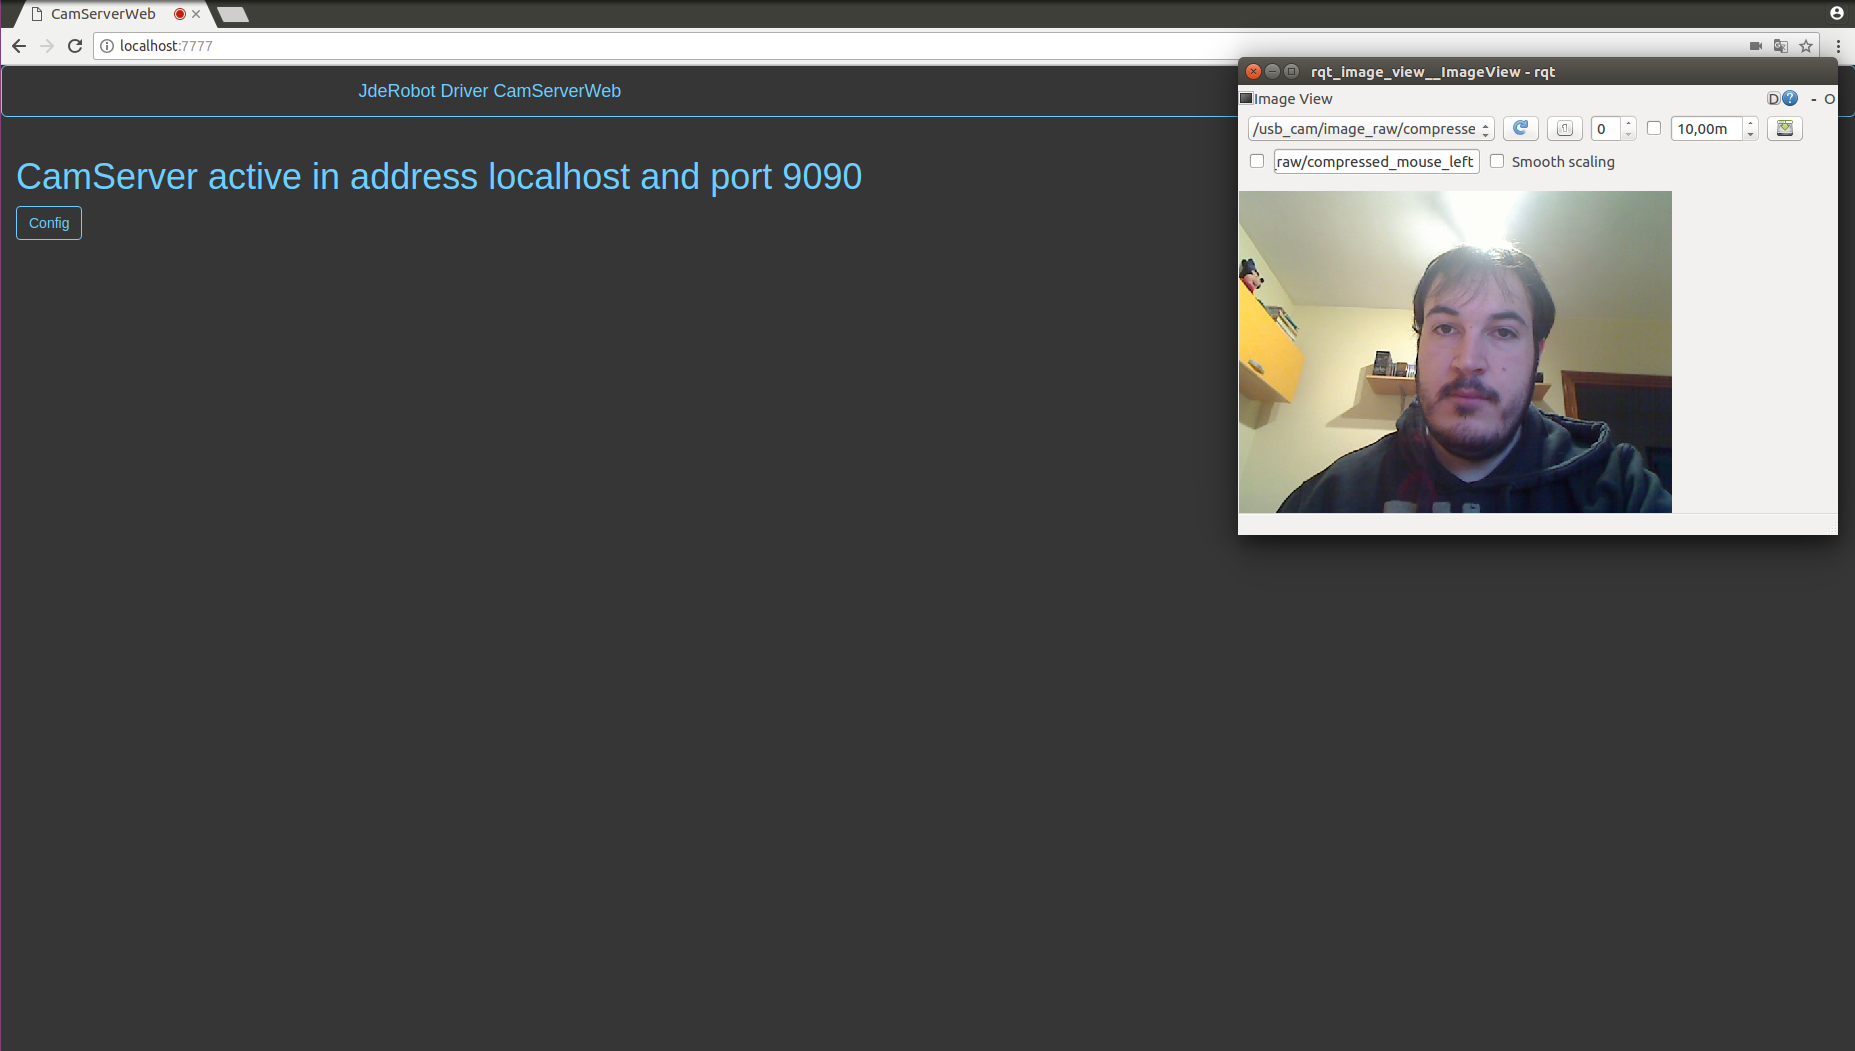
\includegraphics[width=0.4\textwidth]{figures/camservernodejs.png}}
    \subfigure[Electron]{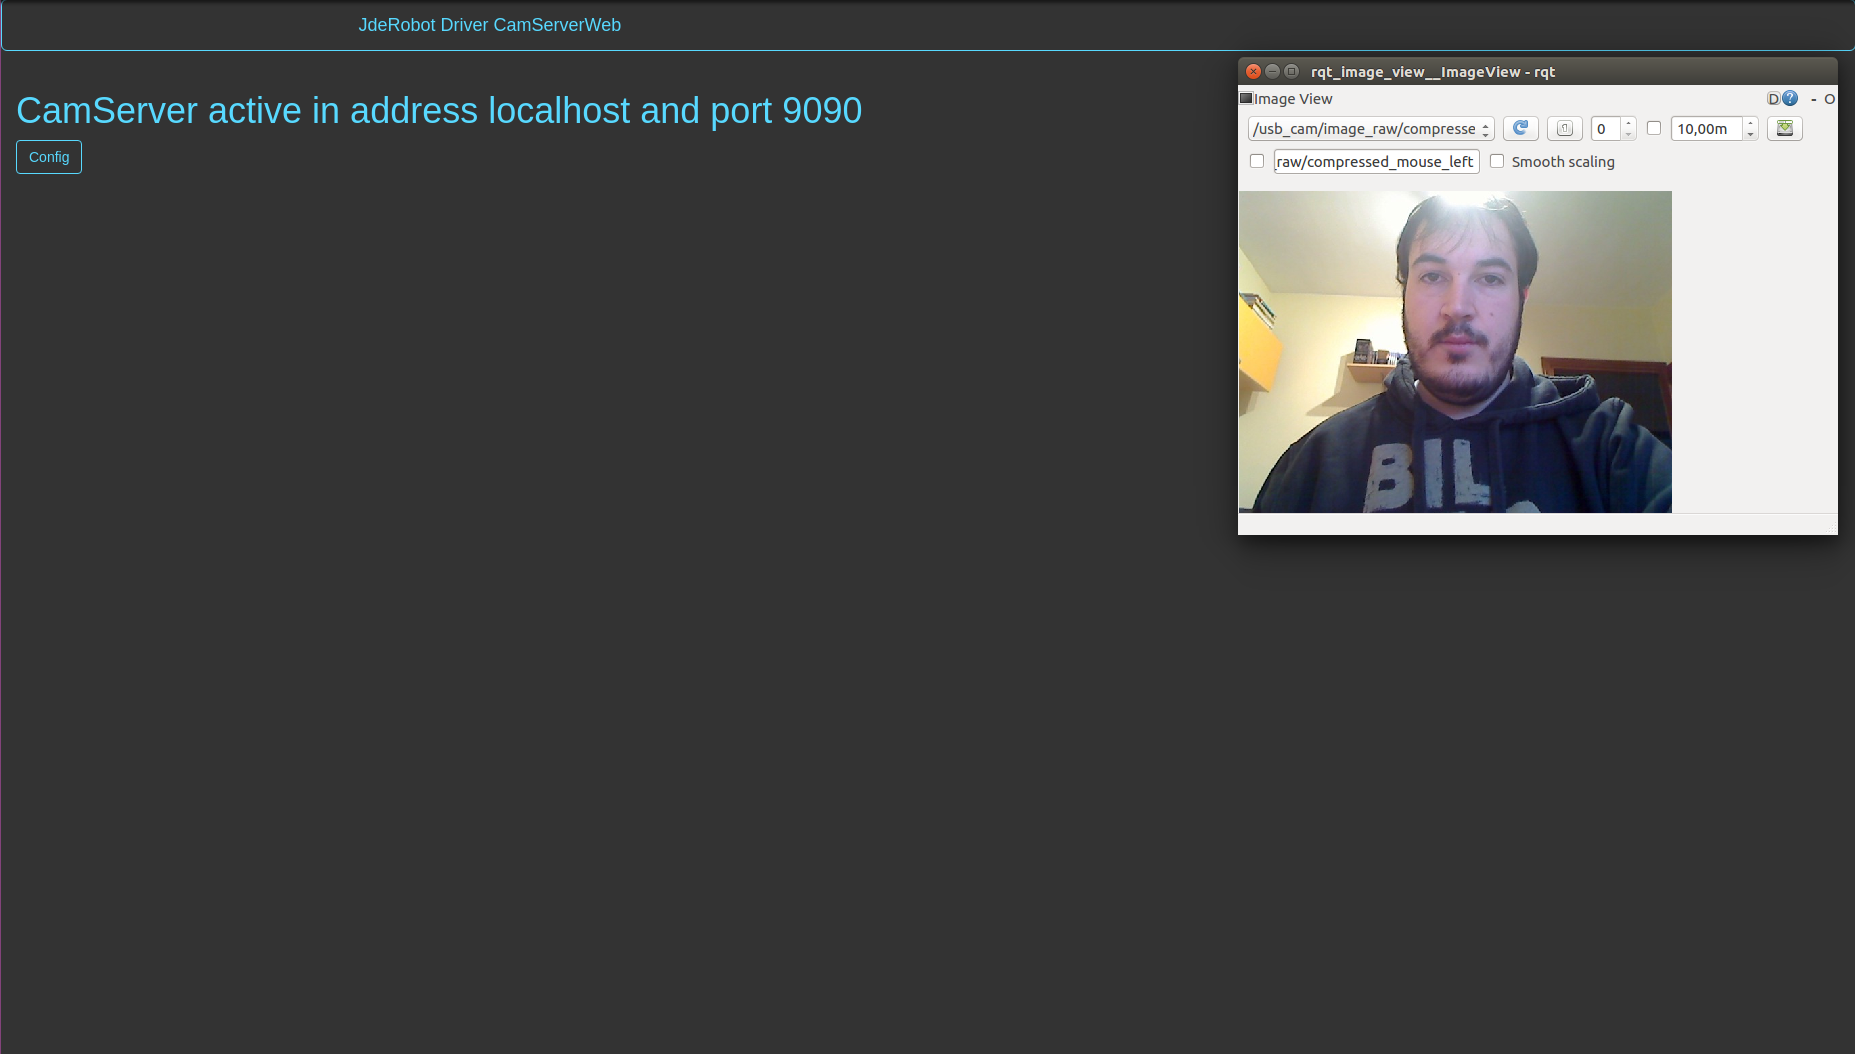
\includegraphics[width=0.4\textwidth]{figures/camserverelectron.png}}
    \caption{camServerWeb ejecutado con Node.js y con Electron}
     \label{fig.ejecuccioncamserver}
     \end{center}
\end{figure}
